\section{Extensions: Reward Alignment with Meta Flow Maps}
\label{sec:extensions}

Beyond unconditional generation, a critical frontier for generative models is the ability to align samples with user-specified rewards or constraints. This task is computationally expensive because it requires estimating the value function $V_t(x) = \log \mathbb{E}[e^{r(X_1)} | X_t = x]$, which in turn demands samples from the conditional posterior $p_{1|t}(x_1 | x_t)$. Traditional methods require costly trajectory rollouts to obtain these posterior samples.

Meta Flow Maps (MFMs) \citep{potaptchik2026meta} address this by extending the deterministic flow map formalism into the \emph{stochastic regime}. A stochastic flow map is defined as a transformation that maps an exogenous noise source $\epsilon$ and an intermediate state $(t, x)$ directly to a sample $x_1 \sim p_{1|t}(\cdot | x)$. By varying the noise input, the map can generate arbitrarily many i.i.d. draws from the posterior in a single step.

\subsection{Training Meta Flow Maps}

MFMs are trained by learning the infinite family of posterior-targeting flow maps simultaneously. The training objective combines two terms:

\textbf{Diagonal loss} (standard flow matching): Enforces the correct instantaneous drift along the diagonal $s=u$:
\begin{equation}
    \mathcal{L}_{\text{diag}} = \int_0^1 \mathbb{E} \| \hat{v}_{u,u}(I_u) - \dot{I}_u \|^2 \, du.
\end{equation}

\textbf{Consistency loss}: Ensures the flow map satisfies the semigroup property globally:
\begin{equation}
    \mathcal{L}_{\text{cons}} = \mathbb{E} \| \hat{X}_{w,u}(\hat{X}_{s,w}(x)) - \hat{X}_{s,u}(x) \|^2.
\end{equation}

\subsection{Value Function Estimation}

The one-step posterior samples provided by MFMs enable efficient estimation of the value function gradient $\nabla V_t(x)$, which is the key quantity for optimal control. Two estimators are available:

\textbf{Gradient-Free Estimator (MFM-GF):} Uses posterior samples $x_1^{(i)} \sim p_{1|t}(\cdot | x)$ and reward evaluations $r(x_1^{(i)})$:
\begin{equation}
    \widehat{\nabla V_t(x)} = \Big(\dot{\beta}_t - \frac{\dot{\alpha}_t}{\alpha_t}\beta_t\Big) \frac{\sum_i x_1^{(i)} e^{r(x_1^{(i)})}}{\sum_i e^{r(x_1^{(i)})}} + \frac{\dot{\alpha}_t}{\alpha_t} x - b_t(x).
\end{equation}

\textbf{Gradient-Based Estimator (MFM-G):} Leverages the reparametrization trick through the differentiable stochastic flow map:
\begin{equation}
    \widehat{\nabla V_t(x)} = \nabla_x \log \Big(\frac{1}{N} \sum_{i=1}^N e^{r(\Phi(\epsilon^{(i)}; t, x))}\Big), \quad \epsilon^{(i)} \sim q.
\end{equation}

These estimators enable two paradigms of control:
\begin{itemize}
    \item \textbf{Inference-time steering:} The value gradient is estimated online at each step and used to modify the sampling drift, directing trajectories toward high-reward states without retraining the model.
    \item \textbf{Training-time fine-tuning:} The value gradient defines a regression target for updating the model parameters, permanently aligning the model with the reward function.
\end{itemize}

Empirically, MFMs achieve competitive sample quality while markedly reducing computation for both steering and fine-tuning, outperforming Best-of-1000 baselines on ImageNet across multiple reward functions at a fraction of the compute. \Cref{alg:meta_flow_maps} outlines the training procedure.

\begin{algorithm}[t]
\caption{Meta Flow Map (MFM) Training}
\label{alg:meta_flow_maps}
\begin{algorithmic}[1]
\Require Data $x_0$, $x_1$, noise $\epsilon$, meta flow map $X_{\text{mfm}}$, optimizer
\State Sample $s, w, u \sim \text{Uniform}(0,1)$ with $s < w < u$
\State Build stochastic interpolants $I_s, I_w, I_u$ with shared $\epsilon$
\State $v_{u,u} \gets X_{\text{mfm}}(I_u, u, u)$ \Comment{Instantaneous velocity (diagonal)}
\State $\dot{I}_u \gets \dot{\alpha}_u \, x_0 + \dot{\beta}_u \, x_1 + \dot{\gamma}_u \, \epsilon$
\State $\mathcal{L}_{\text{diag}} \gets \| v_{u,u} - \dot{I}_u \|^2$ \Comment{Diagonal flow matching loss}
\State $x_w \gets X_{\text{mfm}}(I_s, s, w)$ \Comment{Map $s \to w$}
\State $x_{u}^{\text{composed}} \gets X_{\text{mfm}}(x_w, w, u)$ \Comment{Map $w \to u$}
\State $x_{u}^{\text{direct}} \gets X_{\text{mfm}}(I_s, s, u)$ \Comment{Direct map $s \to u$}
\State $\mathcal{L}_{\text{cons}} \gets \| x_{u}^{\text{composed}} - x_{u}^{\text{direct}} \|^2$ \Comment{Consistency (semigroup) loss}
\State $\mathcal{L} \gets \mathcal{L}_{\text{diag}} + \mathcal{L}_{\text{cons}}$
\State Update parameters with $\nabla \mathcal{L}$
\State \Return $\mathcal{L}$
\end{algorithmic}
\end{algorithm}


\begin{figure}[htbp]
  \centering
  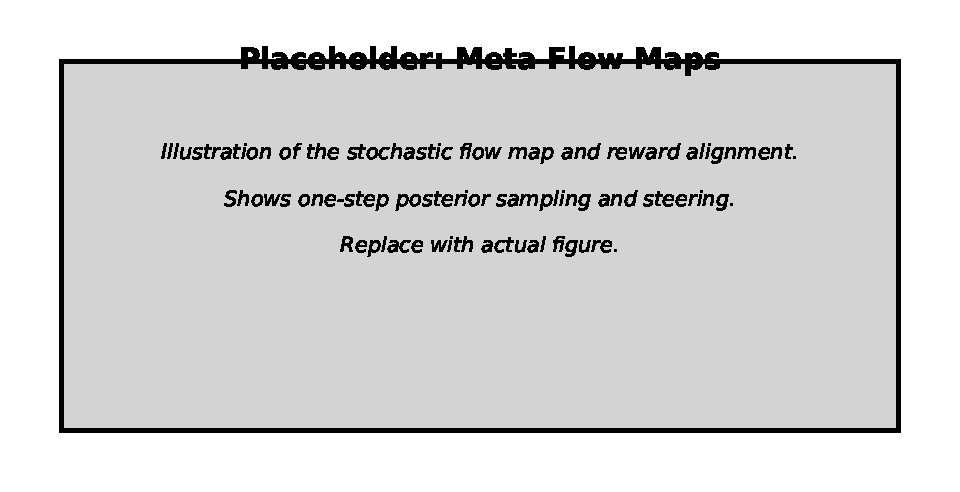
\includegraphics[width=0.8\linewidth]{Figures/figure_meta_flow_maps.pdf}
  \caption{Placeholder: Diagram of a Meta Flow Map showing how a single noise input $\epsilon$ and an intermediate state $(t, x)$ are mapped to a posterior sample $x_1 \sim p_{1|t}(\cdot | x)$. Replace with a figure illustrating the stochastic flow map and reward alignment pipeline.}
  \label{fig:placeholder-meta-flow-maps}
\end{figure}
